\documentclass{beamer}
\usepackage{Freifunkstil}
\begin{document}
\title[Freifunk]{Freifunk - Was ist das?}
\subtitle[Offene Netze]{Wir bauen gemeinsam freie Netze.}
\author{Philipp Schwab \& Emil Foobar}
\date{\today\\\vspace{0.5cm} 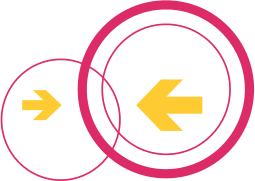
\includegraphics[scale=0.3]{logo-transparent.png}}
\institute{Freifunk Franken}

\begin{frame}
\titlepage	
\end{frame}
\begin{frame}{Inhaltsverzeichnis}
	\tableofcontents
\end{frame}
\section{Kapitel 1}
\begin{frame}{Titel der ersten Folie}
\begin{itemize}
	\item Punkt 1
	\item Punkt 2
\end{itemize}
\end{frame}
\section{Kapitel 2}
\begin{frame}{Titel der zweiten Folie}
	\begin{itemize}
		\item Punkt 1
		\item Punkt 2
	\end{itemize}
\end{frame}
\end{document}